\documentclass{article}
\usepackage[utf8]{inputenc}
\usepackage[T2A]{fontenc}
\usepackage[russian]{babel}
\usepackage{geometry}
\geometry{a4paper, margin=1in}
\usepackage{indentfirst}
\usepackage{amsmath}
\usepackage{graphicx}
\usepackage{listings} 
\usepackage{xcolor} 
\usepackage[colorlinks=false, pdfborder={0 0 0}]{hyperref} 


\lstset{
    breaklines=true,  % Включает перенос длинных строк
}

\begin{document}

\begin{center}
    \textbf{МИНИСТЕРСТВО НАУКИ И ВЫСШЕГО ОБРАЗОВАНИЯ} \\
    \textbf{РОССИЙСКОЙ ФЕДЕРАЦИИ} \\
    \vspace{0.5cm}
    
    \textbf{Федеральное государственное автономное образовательное учреждение} \\
    \textbf{высшего образования} \\
    \vspace{0.5cm}
    
    \textbf{«Национальный исследовательский Нижегородский государственный} \\
    \textbf{университет им. Н.И. Лобачевского»} \\
    \vspace{0.5cm}
    
    \textbf{Институт информационных технологий, математики и механики} \\
    \vspace{0.5cm}
    
    \textbf{Кафедра: Математического обеспечения и суперкомпьютерных технологий} \\
    \vspace{1cm}
    
    Направление подготовки: «Программная инженерия» \\
    Профиль подготовки: «Общий» \\
    \vspace{1cm}
    
    \textit{Отчёт по лабораторной работе на тему:} \\
    \vspace{0.5cm}
    
    \Large\textbf{«Вычисление многомерных интегралов с использованием многошаговой схемы (метод трапеций)»} \\
    \vspace{3.5cm}

    \begin{flushright}
        \textbf{Выполнил:} \\
        студент группы 3822Б1ПP2 \\
        Федоров Матвей \\
        \vspace{1cm}
        
        \textbf{Преподаватель:} \\
         к. т. н. \\
        Сысоев Александр Владимирович \\
        \vspace{0.5cm}
        
        \textbf{Руководитель:} \\
        Нестеров Александр Юрьевич \\
    \end{flushright}
    
    \vfill % Заполняет оставшееся пространство, чтобы текст был внизу
    \small Нижний Новгород \\
    2024
\end{center}

\newpage

\tableofcontents
\newpage

\section{Введение}
Численное интегрирование является важным инструментом в вычислительной математике, позволяющим находить приближенные значения интегралов функций, которые не могут быть вычислены аналитически. Одним из таких методов является метод трапеций, который широко применяется благодаря своей простоте и достаточно высокой точности. Однако при увеличении размерности задачи или необходимости вычисления интегралов с высокой точностью, количество вычислений может значительно возрасти, что приводит к увеличению времени выполнения программы. В современных условиях, когда объемы данных и сложность вычислений постоянно растут, актуальной задачей становится оптимизация алгоритмов численного интегрирования. Одним из эффективных подходов к ускорению вычислений является использование параллельных вычислений, которые позволяют распределить нагрузку между несколькими вычислительными узлами. В данной работе рассматривается реализация последовательного и параллельного алгоритмов метода трапеций для вычисления многомерных интегралов.
   \vspace{1.0cm}
\section{Постановка задачи}
\noindent
\begin{enumerate}
    \item Реализовать последовательную версию задачи по вычислению многомерных интегралов методом трапеций.
    \item Реализовать параллельную версию задачи по вычислению многомерных интегралов методом трапеций.
    \item Подсчитать время работы алгоритмов для последовательной и параллельной задач.
    \item Сравнить результаты подсчётов и сделать выводы об эффективности параллельной версии задачи.
\end{enumerate}
   \vspace{1.0cm}
\section{Математическое обоснование задачи}

\subsection*{Одномерный случай}
Для функции \( f(x) \), заданной на интервале \([a, b]\), интеграл приближенно вычисляется по формуле трапеций:

\[
\int_a^b f(x) \, dx \approx \frac{h}{2} \left( f(a) + 2 \sum_{i=1}^{n-1} f(a + i h) + f(b) \right),
\]

где:
\begin{itemize}
    \item \( h = \frac{b - a}{n} \) — шаг интегрирования,
    \item \( n \) — количество интервалов.
\end{itemize}

\subsection*{Многомерный случай}
Для функции \( f(x_1, x_2, \dots, x_d) \), заданной в \( d \)-мерном пространстве, интеграл по области \( D = [a_1, b_1] \times [a_2, b_2] \times \dots \times [a_d, b_d] \) вычисляется следующим образом:

\[
\int_D f(x_1, x_2, \dots, x_d) \, dx_1 \, dx_2 \dots dx_d \approx \sum_{i_1=0}^{n_1} \sum_{i_2=0}^{n_2} \dots \sum_{i_d=0}^{n_d} w_{i_1, i_2, \dots, i_d} \cdot f(x_{i_1}, x_{i_2}, \dots, x_{i_d}),
\]

где:
\begin{itemize}
    \item \( x_{i_k} = a_k + i_k \cdot h_k \) — точка на \( k \)-м измерении,
    \item \( h_k = \frac{b_k - a_k}{n_k} \) — шаг интегрирования на \( k \)-м измерении,
    \item \( w_{i_1, i_2, \dots, i_d} \) — весовой коэффициент, зависящий от положения точки.
\end{itemize}

\subsection*{Весовые коэффициенты}
Весовые коэффициенты \( w_{i_1, i_2, \dots, i_d} \) определяются следующим образом:
\begin{itemize}
    \item Если точка находится на границе интервала по какому-либо измерению, то вес умножается на \( 1 \).
    \item Если точка находится внутри интервала по всем измерениям, то вес умножается на \( 2 \).
\end{itemize}

Формально:

\[
w_{i_1, i_2, \dots, i_d} = \prod_{k=1}^d w_{i_k},
\]

где:

\[
w_{i_k} = 
\begin{cases}
1, & \text{если } i_k = 0 \text{ или } i_k = n_k, \\
2, & \text{иначе}.
\end{cases}
\]

\subsection*{Итоговая формула}
С учетом весовых коэффициентов и шагов интегрирования, итоговая формула для многомерного метода трапеций принимает вид:

\[
\int_D f(x_1, x_2, \dots, x_d) \, dx_1 \, dx_2 \dots dx_d \approx \frac{h_1 h_2 \dots h_d}{2^d} \sum_{i_1=0}^{n_1} \sum_{i_2=0}^{n_2} \dots \sum_{i_d=0}^{n_d} w_{i_1, i_2, \dots, i_d} \cdot f(x_{i_1}, x_{i_2}, \dots, x_{i_d}).
\]
   \vspace{1.0cm}

\section{Описание алгоритма последовательной задачи}
% Текст описания алгоритма удалён.
\begin{enumerate}
    \item \textbf{Инициализация шага интегрирования:} 
    Для каждого измерения вычисляется шаг интегрирования по формуле:
    \[
    \text{step}[i] = \frac{\text{upper\_bounds}[i] - \text{lower\_bounds}[i]}{\text{intervals}[i]}
    \]
    где \(\text{upper\_bounds}\) и \(\text{lower\_bounds}\) — верхние и нижние границы интегрирования, а \(\text{intervals}\) — количество интервалов для каждого измерения.

    \item \textbf{Рекурсивное вычисление интеграла:} 
    Используется рекурсивная функция \(\text{integrate}\), которая принимает текущую точку в многомерном пространстве и текущее измерение. Если текущее измерение равно размерности задачи, вычисляется значение функции в данной точке с помощью метода \(\text{evaluate\_func}\).

    \item \textbf{Применение метода трапеций:} 
    Для каждого интервала в текущем измерении вычисляется значение функции в начальной и конечной точках (с коэффициентом 1) и в промежуточных точках (с коэффициентом 2). Результаты суммируются и умножаются на шаг интегрирования, деленный на 2:
    \[
    \text{sum} = \sum_{i=0}^{\text{intervals}[d]} \text{value}_i \cdot \text{step}[d] / 2
    \]
    где \(d\) — текущее измерение.

    \item \textbf{Запуск рекурсии:} 
    Рекурсия начинается с начальной точки (все координаты равны 0) и нулевого измерения. Результат рекурсии сохраняется в переменной \(\text{result\_}\).
\end{enumerate}
\section{Описание алгоритма параллельной задачи}
% Текст схемы распараллеливания удалён.
\begin{enumerate}
    \item \textbf{Распределение данных:} 
    Размерность задачи (\(\text{dim}\)), интервалы (\(\text{intervals}\)), нижние (\(\text{lower\_bounds}\)) и верхние (\(\text{upper\_bounds}\)) границы интегрирования передаются от нулевого процесса всем остальным с помощью функции \(\text{boost::mpi::broadcast}\).

    \item \textbf{Вычисление шага интегрирования:} 
    Для каждого измерения вычисляется шаг интегрирования по формуле:
    \[
    \text{step}[i] = \frac{\text{upper\_bounds}[i] - \text{lower\_bounds}[i]}{\text{intervals}[i]}
    \]

    \item \textbf{Распределение нагрузки:} 
    Интервалы интегрирования для первого измерения распределяются между процессами:
    \begin{itemize}
        \item Каждый процесс получает равное количество интервалов.
        \item Остаток распределяется между первыми процессами.
    \end{itemize}
    Границы интегрирования для первого измерения пересчитываются для каждого процесса:
    \[
    \text{lower\_bounds}[0] = \text{rank} \cdot \text{interval\_step}
    \]
    \[
    \text{upper\_bounds}[0] = (\text{rank} + 1) \cdot \text{interval\_step}
    \]
    где \(\text{rank}\) — номер текущего процесса, \(\text{interval\_step}\) — шаг для распределения интервалов.

    \item \textbf{Рекурсивное вычисление интеграла:} 
    Используется рекурсивная функция \(\text{integrate}\), аналогичная последовательной версии. Каждый процесс вычисляет локальный результат для своей части интервала.

    \item \textbf{Сбор результатов:} 
    Локальные результаты всех процессов суммируются с помощью функции \(\text{boost::mpi::reduce}\). Итоговый результат сохраняется на нулевом процессе.

    \item \textbf{Завершение вычислений:} 
    На нулевом процессе итоговый результат умножается на шаг интегрирования и делится на 2:
    \[
    \text{result\_} = \text{global\_result} \cdot \text{step}[0] / 2
    \]
\end{enumerate}
\vspace{1.0cm}

\newpage 

\section{Результаты экспериментов}
\noindent Для сравнения скорости работы последовательной и параллельной реализаций алгоритма применялась следующая тестовая система:
\begin{itemize}
    \item OS: Windows 11
    \item CPU: AMD Ryzen 5 5500U 2.1 GHz
    \item RAM: 16 GB
\end{itemize}
\centering
\subsection*{Результаты тестирования}
\centering
\small\textit{Вычисления производились при нижней границе интегрирования, равной 0.0, при верхней границе интегрирования, равной 1.0, при количестве инервалов, равном 1000000} \\
    \vspace{0.5cm}


% Текст результатов экспериментов удалён.

\centering
\begin{tabular}{|c|c|c|c|}
    \hline
    Число процессов & Вид теста      & Время выполнения (с)  \\ \hline
    1 seq             & pipeline\_run & 12033.0000000000                    \\ \hline
    1 seq             & task\_run     & 0.7159355000                    \\ \hline
    2               & pipeline\_run & 0.7015147000                     \\ \hline
    2               & task\_run     & 0.1401887001                    \\ \hline
    3               & pipeline\_run & 0.4790118999                    \\ \hline
    3               & task\_run     & 0.0690727000                   \\ \hline
    4               & pipeline\_run & 0.4095592999                   \\ \hline
    4               & task\_run     & 0.0510942000                      \\ \hline
    5              & pipeline\_run & 0.3406114000                    \\ \hline
    5              & task\_run     & 0.0384061000                  \\ \hline
    6              & pipeline\_run & 0.3072996001                  \\ \hline
    6              & task\_run     & 0.0370670001                     \\ \hline
    7              & pipeline\_run & 0.2825612001                  \\ \hline
    7              & task\_run     & 0.0343537000                      \\ \hline
    8              & pipeline\_run & 0.2626890000                      \\ \hline
    8            & task\_run     & 0.0313266000                   \\ \hline
\end{tabular}
 \vspace{1.0cm}

\subsection*{График зависимости времени выполнения от числа процессов}
\begin{center}
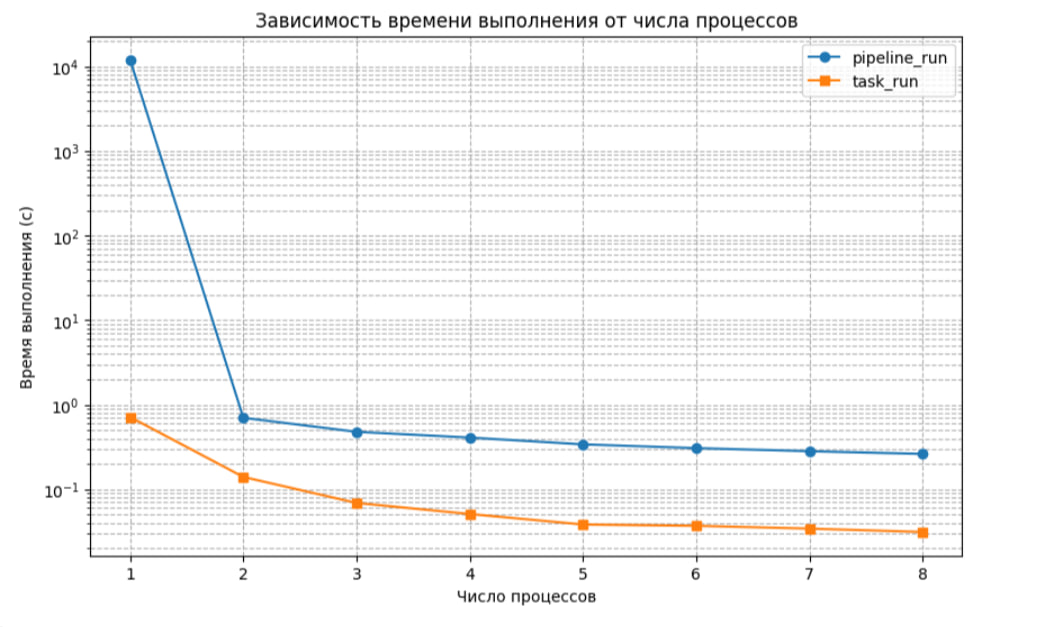
\includegraphics[width=0.8\textwidth]{photo_2024-12-27_15-24-11.jpg}
\end{center}
\raggedright
 \vspace{1cm}

\section{Выводы по результатам экспериментов}

Последовательная версия (\texttt{1 seq}) показала значительно большее время выполнения: 
\begin{itemize}
    \item Для \texttt{pipeline\_run} — \textbf{12033 секунды},
    \item Для \texttt{task\_run} — \textbf{0.7159355 секунды}.
\end{itemize}

Это резко контрастирует с результатами параллельных версий, где время выполнения сокращается до долей секунды уже при использовании \textbf{2 процессов}.

С увеличением числа процессов время выполнения уменьшается. Например:

\begin{itemize}
    \item Для \texttt{pipeline\_run} время снизилось с \textbf{0.7015147 секунды} (2 процесса) до \textbf{0.2626890 секунды} (8 процессов).
    \item Для \texttt{task\_run} время снизилось с \textbf{0.1401887 секунды} (2 процесса) до \textbf{0.0313266 секунды} (8 процессов).
\end{itemize}

Что свидетельствует о том, что параллельная реализация позволяет существенно сократить время выполнения задачи и эффективно распределяет нагрузку между процессами.

 \vspace{1.0cm}
 
\section{Заключение}
% Текст заключения удалён.

\hspace{0.5cm}В данной работе были разработаны и сравнены последовательная и параллельная версии алгоритма вычисления многомерных интегралов методом трапеций. Параллельная реализация, использующая MPI, показала значительное сокращение времени вычислений по сравнению с последовательной, особенно при увеличении числа задействованных процессов. Это подчеркивает эффективность MPI для распараллеливания задач численного интегрирования.

 \vspace{1cm}

 \section{Литература}
\begin{itemize}
    \item C++ и Численные Методы: Приближенное интегрирование по Ньютону-Котесу: \url{https://habr.com/ru/articles/479202/}
    \item Limit of Integration: \url{https://www.geeksforgeeks.org/limit-of-integration/}
    \item Формула трапеции: \url{https://math.semestr.ru/optim/trapezoid-formula.php}
\end{itemize}

\vspace{1cm}


\section{Приложение}
\subsection{ops\_seq.hpp}
\begin{lstlisting}[language=C++]
#pragma once

#include <gtest/gtest.h>

#include <boost/mpi/collectives.hpp>
#include <boost/mpi/communicator.hpp>
#include <boost/serialization/vector.hpp>
#include <memory>
#include <numeric>
#include <string>
#include <utility>
#include <vector>

#include "core/task/include/task.hpp"

namespace fyodorov_m_trapezoidal_method_mpi {

class TestTaskSequential : public ppc::core::Task {
 public:
  explicit TestTaskSequential(std::shared_ptr<ppc::core::TaskData> taskData_) : Task(std::move(taskData_)) {}
  bool pre_processing() override;
  bool validation() override;
  bool run() override;
  bool post_processing() override;

 private:
  std::function<double(const std::vector<double>&)> func_;
  std::vector<double> lower_bounds_;
  std::vector<double> upper_bounds_;
  std::vector<int> intervals_;
  double result_{};

  static double evaluate_func_sequential(const std::function<double(const std::vector<double>&)>& func,
                                         const std::vector<double>& point);
};

// namespace fyodorov_m_trapezoidal_method_seq

class TestMPITaskParallel : public ppc::core::Task {
 public:
  explicit TestMPITaskParallel(std::shared_ptr<ppc::core::TaskData> taskData_,
                               std::function<double(const std::vector<double>&)> func)
      : Task(std::move(taskData_)), func_(std::move(func)) {}
  bool pre_processing() override;
  bool validation() override;
  bool run() override;
  bool post_processing() override;

 private:
  std::function<double(const std::vector<double>)> func_;
  std::vector<double> lower_bounds_;
  std::vector<double> upper_bounds_;
  std::vector<int> intervals_;
  double result_{};
  boost::mpi::communicator world;
  static double evaluate_func_parallel(const std::function<double(const std::vector<double>&)>& func,
                                       const std::vector<double>& point);
};

}  // namespace fyodorov_m_trapezoidal_method_mpi
\end{lstlisting}

% Текст приложения 7.1 удалён.

\subsection{ops\_seq.cpp}
% Текст приложения 7.2 удалён.
\begin{lstlisting}[language=C++]
#include "seq/fyodorov_m_trapezoidal_method_seq/include/ops_seq.hpp"

#include <iostream>
#include <numeric>
#include <thread>

using namespace std::chrono_literals;

double fyodorov_m_trapezoidal_method_seq::TestTaskSequential::evaluate_func(
    const std::function<double(const std::vector<double>&)>& func, const std::vector<double>& point) {
  return func(point);
}

bool fyodorov_m_trapezoidal_method_seq::TestTaskSequential::pre_processing() {
  internal_order_test();
  // Init value for input and output
  if (taskData->inputs_count.size() < 4) return false;  //

  func_ = *reinterpret_cast<std::function<double(const std::vector<double>&)>*>(taskData->inputs[0]);

  size_t dim = taskData->inputs_count[1];
  lower_bounds_.resize(dim);
  upper_bounds_.resize(dim);
  intervals_.resize(dim);

  for (size_t i = 0; i < dim; ++i) {
    lower_bounds_[i] = reinterpret_cast<double*>(taskData->inputs[1])[i];
    upper_bounds_[i] = reinterpret_cast<double*>(taskData->inputs[2])[i];
    intervals_[i] = reinterpret_cast<int*>(taskData->inputs[3])[i];
  }
  result_ = 0.0;
  return true;
}

bool fyodorov_m_trapezoidal_method_seq::TestTaskSequential::validation() {
  internal_order_test();
  if (taskData->outputs_count.size() != 1 || taskData->outputs_count[0] != 1) {
    return false;
  }

  
  for (size_t i = 0; i < lower_bounds_.size(); ++i) {
    if (lower_bounds_[i] >= upper_bounds_[i]) {
      return false;
    }
  }

  
  for (size_t i = 0; i < intervals_.size(); ++i) {
    if (intervals_[i] <= 0) {
      return false;
    }
  }

  return true;
}

bool fyodorov_m_trapezoidal_method_seq::TestTaskSequential::run() {
  internal_order_test();

  size_t dim = lower_bounds_.size();
  std::vector<double> step(dim);
  for (size_t i = 0; i < dim; ++i) step[i] = (upper_bounds_[i] - lower_bounds_[i]) / intervals_[i];

  std::function<double(std::vector<double>, size_t)> integrate = [&](std::vector<double> current_point,
                                                                     size_t current_dim) -> double {
    if (current_dim == dim) {
      return evaluate_func(func_, current_point);
    }
    double sum = 0.0;
    for (int i = 0; i <= intervals_[current_dim]; ++i) {
      current_point[current_dim] = lower_bounds_[current_dim] + i * step[current_dim];
      double value;
      if (i == 0 || i == intervals_[current_dim]) {
        value = integrate(current_point, current_dim + 1);
      } else {
        value = 2 * integrate(current_point, current_dim + 1);
      }
      sum += value;
    }
    return sum * step[current_dim] / 2.0;
  };
  std::vector<double> start_point(dim, 0.0);
  result_ = integrate(start_point, 0);
  return true;
}

bool fyodorov_m_trapezoidal_method_seq::TestTaskSequential::post_processing() {
  std::cout << "pre_processing() called" << std::endl;
  internal_order_test();
  reinterpret_cast<double*>(taskData->outputs[0])[0] = result_;
  return true;
}
\end{lstlisting}
\subsection{ops\_mpi.hpp}
% Текст приложения 7.3 удалён.
\begin{lstlisting}[language=C++]

#pragma once

#include <gtest/gtest.h>

#include <boost/mpi/collectives.hpp>
#include <boost/mpi/communicator.hpp>
#include <boost/serialization/vector.hpp>
#include <memory>
#include <numeric>
#include <string>
#include <utility>
#include <vector>

#include "core/task/include/task.hpp"

namespace fyodorov_m_trapezoidal_method_mpi {

class TestTaskSequential : public ppc::core::Task {
 public:
  explicit TestTaskSequential(std::shared_ptr<ppc::core::TaskData> taskData_) : Task(std::move(taskData_)) {}
  bool pre_processing() override;
  bool validation() override;
  bool run() override;
  bool post_processing() override;

 private:
  std::function<double(const std::vector<double>&)> func_;
  std::vector<double> lower_bounds_;
  std::vector<double> upper_bounds_;
  std::vector<int> intervals_;
  double result_{};

  static double evaluate_func_sequential(const std::function<double(const std::vector<double>&)>& func,
                                         const std::vector<double>& point);
};

// namespace fyodorov_m_trapezoidal_method_seq

class TestMPITaskParallel : public ppc::core::Task {
 public:
  explicit TestMPITaskParallel(std::shared_ptr<ppc::core::TaskData> taskData_,
                               std::function<double(const std::vector<double>&)> func)
      : Task(std::move(taskData_)), func_(std::move(func)) {}
  bool pre_processing() override;
  bool validation() override;
  bool run() override;
  bool post_processing() override;

 private:
  std::function<double(const std::vector<double>)> func_;
  std::vector<double> lower_bounds_;
  std::vector<double> upper_bounds_;
  std::vector<int> intervals_;
  double result_{};
  boost::mpi::communicator world;
  static double evaluate_func_parallel(const std::function<double(const std::vector<double>&)>& func,
                                       const std::vector<double>& point);
};

}  // namespace fyodorov_m_trapezoidal_method_mpi

\end{lstlisting}
\subsection{ops\_mpi.cpp}
% Текст приложения 7.4 удалён.
\begin{lstlisting}[language=C++]
#include "mpi/fyodorov_m_trapezoidal_method_mpi/include/ops_mpi.hpp"

#include <algorithm>
#include <boost/mpi.hpp>
#include <boost/mpi/collectives.hpp>
#include <boost/mpi/communicator.hpp>
// #include <boost/serialization/access.hpp>
// #include <boost/serialization/vector.hpp>
#include <functional>
#include <string>
#include <thread>
#include <vector>

bool fyodorov_m_trapezoidal_method_mpi::TestTaskSequential::pre_processing() {
  internal_order_test();
  // Init value for input and output
  if (taskData->inputs_count.size() < 4) return false;  //

  func_ = *reinterpret_cast<std::function<double(const std::vector<double>&)>*>(taskData->inputs[0]);

  size_t dim = taskData->inputs_count[1];
  lower_bounds_.resize(dim);
  upper_bounds_.resize(dim);
  intervals_.resize(dim);

  for (size_t i = 0; i < dim; ++i) {
    lower_bounds_[i] = reinterpret_cast<double*>(taskData->inputs[1])[i];
    upper_bounds_[i] = reinterpret_cast<double*>(taskData->inputs[2])[i];
    intervals_[i] = reinterpret_cast<int*>(taskData->inputs[3])[i];
  }
  result_ = 0.0;
  return true;
}

bool fyodorov_m_trapezoidal_method_mpi::TestTaskSequential::validation() {
  internal_order_test();

  if (taskData->outputs_count.size() != 1 || taskData->outputs_count[0] != 1) {
    return false;
  }

  
  for (size_t i = 0; i < lower_bounds_.size(); ++i) {
    if (lower_bounds_[i] >= upper_bounds_[i]) {
      return false;
    }
  }

  for (size_t i = 0; i < intervals_.size(); ++i) {
    if (intervals_[i] <= 0) {
      return false;
    }
  }

  return true;
}

bool fyodorov_m_trapezoidal_method_mpi::TestTaskSequential::run() {
  internal_order_test();

  size_t dim = lower_bounds_.size();
  std::vector<double> step(dim);
  for (size_t i = 0; i < dim; ++i) step[i] = (upper_bounds_[i] - lower_bounds_[i]) / intervals_[i];

  std::function<double(std::vector<double>, size_t)> integrate = [&](std::vector<double> current_point,
                                                                     size_t current_dim) -> double {
    if (current_dim == dim) {
      return func_(current_point);
    }
    double sum = 0.0;
    for (int i = 0; i <= intervals_[current_dim]; ++i) {
      current_point[current_dim] = lower_bounds_[current_dim] + i * step[current_dim];
      double value;
      if (i == 0 || i == intervals_[current_dim]) {
        value = integrate(current_point, current_dim + 1);
      } else {
        value = 2 * integrate(current_point, current_dim + 1);
      }
      sum += value;
    }
    return sum * step[current_dim] / 2.0;
  };
  std::vector<double> start_point(dim, 0.0);
  result_ = integrate(start_point, 0);
  return true;
}

bool fyodorov_m_trapezoidal_method_mpi::TestTaskSequential::post_processing() {
  internal_order_test();
  reinterpret_cast<double*>(taskData->outputs[0])[0] = result_;
  return true;
}

// Implementation for parallel task

bool fyodorov_m_trapezoidal_method_mpi::TestMPITaskParallel::pre_processing() {
  internal_order_test();

  world = boost::mpi::communicator();
  // Init value for input and output
  if (world.rank() == 0) {
    if (taskData->inputs_count.size() < 3) return false;  //

    size_t dim = taskData->inputs_count[1];
    lower_bounds_.resize(dim);
    upper_bounds_.resize(dim);
    intervals_.resize(dim);

    for (size_t i = 0; i < dim; ++i) {
      lower_bounds_[i] = reinterpret_cast<double*>(taskData->inputs[0])[i];
      upper_bounds_[i] = reinterpret_cast<double*>(taskData->inputs[1])[i];
      intervals_[i] = reinterpret_cast<int*>(taskData->inputs[2])[i];
    }

    result_ = 0.0;
  }
  return true;
}

bool fyodorov_m_trapezoidal_method_mpi::TestMPITaskParallel::validation() {
  internal_order_test();

  for (size_t i = 0; i < lower_bounds_.size(); ++i) {
    if (lower_bounds_[i] >= upper_bounds_[i]) {
      return false;
    }
  }

  for (size_t i = 0; i < intervals_.size(); ++i) {
    if (intervals_[i] <= 0) {
      return false;
    }
  }

  if (world.rank() == 0) {
    return taskData->outputs_count[0] == 1;
  }

  return true;
}

bool fyodorov_m_trapezoidal_method_mpi::TestMPITaskParallel::run() {
  internal_order_test();

  size_t dim = (world.rank() == 0) ? lower_bounds_.size() : 0;
  boost::mpi::broadcast(world, dim, 0);
  boost::mpi::broadcast(world, intervals_, 0);
  boost::mpi::broadcast(world, lower_bounds_, 0);
  boost::mpi::broadcast(world, upper_bounds_, 0);

  std::vector<double> step(dim);
  for (size_t i = 0; i < dim; i++) step[i] = (upper_bounds_[i] - lower_bounds_[i]) / intervals_[i];

  if (dim > 0) {
    int interval_per_process = intervals_[0] / world.size();
    int remainder = intervals_[0] % world.size();

    intervals_[0] = interval_per_process + (world.rank() < remainder ? 1 : 0);
    double interval_step = (upper_bounds_[0] - lower_bounds_[0]) / world.size();
    lower_bounds_[0] = world.rank() * interval_step;
    upper_bounds_[0] = (world.rank() + 1) * interval_step;
  }

  std::function<double(std::vector<double>, size_t)> integrate = [&](std::vector<double> current_point,
                                                                     size_t current_dim) -> double {
    if (current_dim == dim) {
      return func_(current_point);
    }
    double sum = 0.0;
    for (int i = 0; i <= intervals_[current_dim]; ++i) {
      current_point[current_dim] = lower_bounds_[current_dim] + i * step[current_dim];
      double value;
      if (i == 0 || i == intervals_[current_dim]) {
        value = integrate(current_point, current_dim + 1);
      } else {
        value = 2 * integrate(current_point, current_dim + 1);
      }
      sum += value;
    }
    return sum * step[current_dim] / 2.0;
  };

  std::vector<double> start_point = lower_bounds_;
  double local_result = 0;

  for (int i = 0; i <= intervals_[0]; i++) {
    start_point[0] = lower_bounds_[0] + i * step[0];
    double value;
    if (i == 0 || i == intervals_[0]) {
      value = integrate(start_point, 1);
    } else {
      value = 2 * integrate(start_point, 1);
    }
    local_result += value;
  }

  double global_result = 0.0;
  boost::mpi::reduce(world, local_result, global_result, std::plus<>(), 0);

  if (world.rank() == 0) {
    result_ = global_result * step[0] / 2.0;
  }

  return true;
}

bool fyodorov_m_trapezoidal_method_mpi::TestMPITaskParallel::post_processing() {
  internal_order_test();
  if (world.rank() == 0) {
    reinterpret_cast<double*>(taskData->outputs[0])[0] = result_;
  }
  return true;
}

\end{lstlisting}
\end{document}
